%\lecture{4}{Tue 28 Jan 2020 14:44}{393 Lab 3}
\section{Response Characteristics}
\begin{table}[H]
	\centering
	\caption{Varied $P$-value}
\begin{tabular}{ | | c c c c c | | }
P Value & Overshoot & Rise Time & Settling Time & Steady State Error \\
\hline \hline
1       & None      & n/a       & 0.4 s         & - 1.1              \\
5       & 10.98     & 0.148 s   & 0.36 s        & + 0.018            \\
10      & 11.08     & 0.15 s    & 0.45 s        & + 0.007            \\
20      & 11.23     & 0.148 s   & 0.61 s        & None              
\end{tabular}
\end{table}

Our chosen, "ideal" $P$-value was found to be 20.% todo: insert the chosen ideal p value 

\begin{table}[H]
	\centering
	\caption{Varied $D$-value}
\begin{tabular}{ | | c c c c c | | }
D Value & Overshoot & Rise Time & Settling Time & Steady State Error \\
\hline \hline
0.01    & 11.129    & 0.148 s   & 0.61 s        & None               \\
0.03    & 11.08     & 0.17 s    & 0.59 s        & - 0.0015           \\
0.1     & 10.7      & 0.148 s   & 0.37 s        & - 0.0015           \\
0.3     & 10.007    & 0.21 s    & 0.35 s        & - 0.0015           \\
0.7     & None      & 0.3 s     & 0.48 s        & + 0.02 to - 0.03   \\
1       & 10.0537   & 0.36 s    & 0.53 s        & + 0.07 to - 0.09  
\end{tabular}
\end{table}

Our chosen, "ideal" $D$-value was found to be 0.3.

\begin{table}[H]
	\centering
	\caption{Varied $I$-value}
\begin{tabular}{ | | c c c c c | | }
I Value & Overshoot & Rise Time & Settling Time & Steady State Error \\
\hline \hline
0.001   & 10.0016   & 0.21 s    & 0.336 s       & - 0.003            \\
0.08    & 10.0031   & 0.306 s   & 0.336 s       & + 0.0031           \\
0.3     & 10.0261   & 0.204 s   & 0.372 s       & + 0.0138           \\
1       & 10.049    & 0.20 s    & 0.37 s        & + 0.043           
\end{tabular}
\end{table}


\section{Varying P, I, and D}
\subsection{P Value}
As \(P\) increased, the steady state error decreased until it was zero with \(P = 20\). Increasing \(P\) also led to higher overshoot, and a higher settling time, as the response had more oscillations around the target value before reaching steady state.
\subsection{I Value}
As \(I\) increased, the steady state error and overshoot both increased. The rise time was mostly unchanged except for \(I = 0.08\), but it was highly variable due to the nature of the oscillating response. The settling time was essentially unchanged with different values of I.
\subsection{D Value}
As \(D\) increased, the steady state error increased and the steady state became more oscillatory. The rise time increased as the system began to oscillate more before reaching the maximum value as it was anticipating overshooting. The overshoot was a minimum at \(D = 0.7\). We chose \(D = 0.3\) as our optimal value as it had a consistent low steady state error and minimal overshoot.

\section{Consistent Oscillations}
\begin{figure}[H]
	\centering
	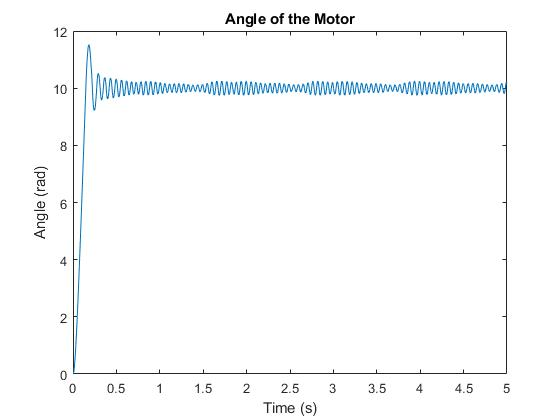
\includegraphics[width=0.8\textwidth]{./figures/lab3_P_only_osscilation.jpg}
	\caption{Oscillation around target value of 10 rads with $P = 50$. }
	\label{fig:Oscillation}
\end{figure}
% todo: include fig 2  
By setting \(P = 50, I = 0, D = 0\), the motor oscillated around the target value of \(10 \) rads, as seen in Figure \ref{fig:Oscillation}. As P increases, the imaginary portion of the poles of the transfer function tend towards positive and negative infinity, while the real component tends towards zero (from the negative side). The large magnitude of the complex component corresponds to higher amplitude sinusoidal response.

\section{Output with Only Integral Control}
\begin{figure}[H]
	\centering
	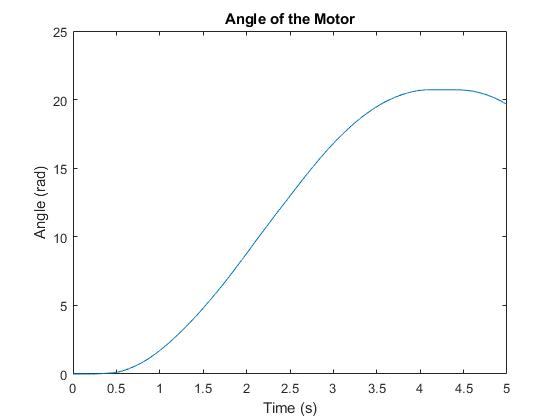
\includegraphics[width=0.8\textwidth]{./figures/lab3_10rad_oscillations.jpg}

	\caption{Plot of Output with Only Integral Control}
	\label{fig:int}
\end{figure}
The poles of the transfer function, using the values \(P = 0, I = 0.08, D = 0\) results in \(s = 0.01 \pm 0.76i\), shown above in Figure \ref{fig:int}. This has a very small (but positive) real component, which indicates that the system will tend towards instability as \(t \Rightarrow \infty\). This was more evident when the simulation was ran with \(P=0, D=0, I=1\), which produced Figure \ref{fig:unstable} below:
\begin{figure}[H]
	\centering
	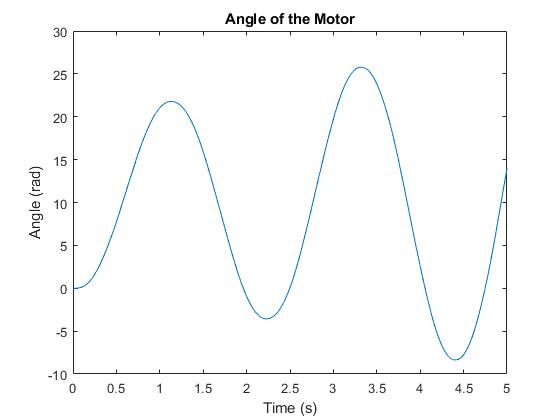
\includegraphics[width=0.8\textwidth]{./figures/lab3_integral_unstable.jpg}
	\caption{Very unstable transfer function using only $I$ value}
	\label{fig:unstable}
\end{figure}
The output with only integral control is an unstable solution. 

\section{Plot with Desired Angle}
The chosen $P$, $I$ and $D$ values for our best control system were found to be \(P = 20, I = 0.08, D = 0.3\). 

The "interesting" function our control system mirrored is shown in Figure \ref{fig:interesting}. 
\begin{figure}[H]
	\centering
	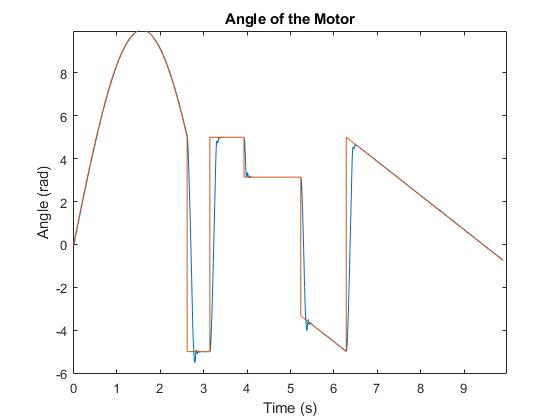
\includegraphics[width=0.8\textwidth]{./figures/lab3_custom_function.jpg}
	\caption{A custom function generated in Simulink}
	\label{fig:interesting}
\end{figure}
